\newcommand{\smallProfile}[1]
{%
	\begin{tikzpicture}
	\begin{axis}[		
		no markers,
		scale only axis,
		width=\linewidth,
		height=0.5\linewidth,
		xtick=\empty,
		ytick=\empty,
		enlargelimits=false
	]

	\addplot table[x=Index,y=Value] {#1};

	\end{axis}
	\end{tikzpicture}%
}




\chapter{1D Edge Detection} 
\label{chap:1DEdgeDetection}

\epigraph{The edge... There is no honest way to explain it because the only people who really know where it is are the ones who have gone over.}
{\textsc{Hunter S. Thompson}}

\pagebreak

\section{Introduction}
\paragraph*{}
Image edges are locations of sharp change of brightness, i.e. locations of high local contrast. As a consequence of being a contrast-based feature, the presence and position of an edge is not altered by global illumination changes in the image; which contributes to the robustness of Edge Detection-based solutions.

\paragraph*{}
Edge detection techniques come in two variants depicted in \reffig{1D2DEdges}. \textbf{1D~Edge Detection} methods scan the image along a path and locate the points of intersection between image edges and the scan line. \textbf{2D~Edge Detection} methods locate the entire edge. In this chapter we will inspect the first technique, featuring remarkable performance and sub-pixel precision.

\twoFigures
{img/1DEdgeDetection/edge1D}
{img/1DEdgeDetection/edge2D}
{\textbf{1D Edge Detection}, \textbf{2D Edge Detection}}
{1D2DEdges}
{\basicWidth}

\paragraph*{}
We will start with a short description of the methodology of extracting a 1D image brightness profile along a given path and then proceed to detection of the features present in the profile.

\paragraph*{}
Depending on the nature of the brightness change that constitutes an edge, we distinguish two kinds of edges: \textbf{step edges}, occurring between two areas of different intensity, and \textbf{ridge edges} (or simply ridges), occurring where image intensity changes briefly and then returns to initial value.

\paragraph*{}
A wide class of visual inspection tasks is focused on the areas bounded by two step edges of opposite polarity, rather than on the edges considered separately. Because of that it is useful to consider such areas as a third, additional type of feature discernible in one-dimensional profile; here called a \textbf{stripe}.  

\paragraph*{}
Overall, the chapter will cover detection of three kinds of features discernible in 1D profiles, all demonstrated in \reftab{1DFeatures}. In each example the feature (step edge, ridge or stripe) is vertical and the image is scanned horizontally to find the points of intersection between the feature and the scan line.

\begin{table}[h]
\centering
\begin{tabular}{c c c}
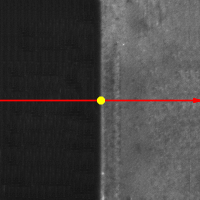
\includegraphics[width=0.275\textwidth]{img/1DEdgeDetection/edge}
& 
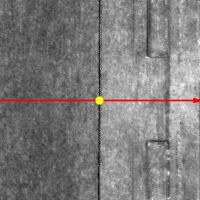
\includegraphics[width=0.275\textwidth]{img/1DEdgeDetection/ridge}
&
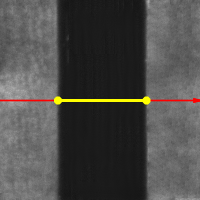
\includegraphics[width=0.275\textwidth]{img/1DEdgeDetection/stripe}
\\
\textbf{Step Edge} &
\textbf{Ridge} &
\textbf{Stripe} 
\end{tabular}
\caption{Different kinds of image features extracted from 1D profile.}
\label{tab:1DFeatures}
\end{table}
\section{Profile Extraction}

\paragraph*{}
Before we apply any of the \textbf{1D Edge Detection} methods, firstly we need to acquire a 1D profile that is to be inspected. Computing a discrete profile of image brightness along a given path is relatively straightforward task.

\paragraph*{}
The first step is to sample the scan path, selecting a set of equidistant (typically with distance of one pixel \cite[p. 150]{MVTec08}) points of interest along the path. Each of these points will correspond to one element of the constructed profile. The second step is to compute the brightness values \textit{related to} each of the points.

\subsection{Multiple Sampling}
\paragraph*{}
We used the expression \textit{related to} rather than \textit{at} on purpose - although we could simply take the image brightness values at each point of interest, it is more prudent to use an average of a series of sampling points perpendicular to the scan line, as demonsted in \reffig{MultipleSampling}; thus achieving a simple mean of noise suppression. But what kind of average should we use to compute the result for a single point of interest?

\oneFigure
{img/1DEdgeDetection/multiple_sampling_refined}
{Multiple Sampling for 1D Edge Detection.}
{MultipleSampling}
{\basicWidth}

\paragraph*{}
As long as the whole range of sampling points fits within the object being inspected and its features are perpendicular to the scan path, the brightness information collected at each of the sampling points is equally good or bad as the information collected at the other ones. Because of that we may safely use the simplest arithmetic mean.

\paragraph*{}
We will refer to the number of points used to compute a single profile value as \textit{scan width}. The wider the scan, the stronger noise attenuation we get. However, if the 2D feature we are to inspect is not perfectly perpendicular to the scan line, the wide scan area will cause the edge in the resulting 1D profile to be stretched and thus harder to identify precisely. Increasing the scan width will also increase the computation time of the profile extraction, which depends linearly on the number of sampling points.

\paragraph*{}
\reffig{EdgesProfileExtraction} demonstrates an example brightness profile extracted from the image on the right, scanned horizontally along the red scan line.

\begin{figure}[h!]
    \begin{subfigure}[b]{\basicWidth}
		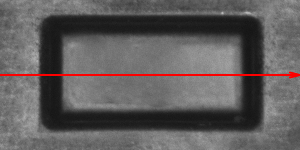
\includegraphics[width=\linewidth]{img/1DEdgeDetection/edges_scan}
    \end{subfigure}%
    ~
    \begin{subfigure}[b]{\basicWidth}
		\smallProfile{img/1DEdgeDetection/edge_profile.values}
    \end{subfigure}
    \caption{1D brightness profile extracted from the image.}
    \label{fig:EdgesProfileExtraction}
\end{figure}

\subsection{Refinement}

\paragraph*{}
Even though reasonably wide scan area suppresses the noise significantly at the extraction level, we need to keep in mind that only random noise can be suppressed in this way. Real pictures contain small features\footnote{Possibly perpendicular to the scan line and thus not affected by averaging the sampling points.} of image texture irrelevant to the inspection task that need to be attenuated before further processing of the profile. 

\paragraph*{}
Selecting the smoothing filter to refine the extracted profile is not an obvious choice. On the one hand we want to suppress the noise present in the profile, so that irrelevant intensity changes are not identified as edge points, on the other hand we want to achieve high precision of the edge localization. 

\paragraph*{}
These two criteria cannot be considered independently - smoothing of the profile suppresses the noise, but also lowers the precision. Canny determined\cite{Canny86} that the optimal trade-off between noise reduction and lose of precision is achieved with the Gaussian smoothing filter defined as follows:

\[
    g_{\sigma}(x)= \frac{1}{\sqrt{2\pi \sigma^2}} e^{-\frac{x^2}{2 \sigma^2}}
\]

where the standard deviation $\sigma$ is a parameter of the filter.

\subsubsection{Discreet Gaussian Filter}

\paragraph*{}
The Gaussian function is defined in continuous, infinite domain - to obtain a discreet approximation of the filter, we may sample $g_{\sigma}(x)$ at integer coordinates\cite{JainKasturi95}. Moreover, as the value of the Gaussian function quickly decreases with the increase of $|x|$, we may limit the discreet filter to a finite neighborhood of $x = 0$ without significant effect on the results of the smoothing. 

\paragraph*{}
The well known fact called a three-sigma rule states that more that $97\%$ of the Gaussian function integral is concentrated within $3 \sigma$ distance from $x = 0$. It is therefore reasonable to sample the Gaussian function at $2r + 1$ points, where $r$ is a small multiple of $\sigma$, e.g. $3 \lceil \sigma \rceil$; thus obtaining a mask in the following form:

\[
    \frac{1}{s} \begin{bmatrix}
    g(r) & g(r-1) & ... & g(0) & ... & g(r-1) & g(r) 
    \end{bmatrix}
\]

where $s$ equals the sum of the obtained gaussian coefficients, i.e. it ensures the mean-preservation property of the filter.

\subsubsection{Standard Deviation}

\paragraph*{}
Accurate adjustment of $\sigma$ will contribute to the robustness of the computation. We should pick a value that is high enough to eliminate noise that could introduce irrelevant extrema to the profile derivative, but low enough to preserve the actual edges we are to detect. This parameter should be adjusted through interactive experimentation on representative sample data, looking for optimal trade-off between fidelity and noise attenuation. 

\paragraph*{}
\reffig{ProfileSmoothingStdDev} demonstrates effects of smoothing the example brightness profile with different $\sigma$ values. Blue profile ($\sigma = 0.0$) exhibits fine noise while brown profile ($\sigma = 6.0$) attenuates the valleys of significant edges, which makes both suboptimal. Red profile ($\sigma = 3.0$) seems to exhibit appropriate degree of smoothing.

\profileFigure
{
	\addProfileData{img/1DEdgeDetection/edge_profile.values}
	\addProfileData{img/1DEdgeDetection/edge_profile_low_smoothing.values}
	\addProfileData{img/1DEdgeDetection/edge_profile_high_smoothing.values}
}
{Original brightness profile smoothed with different standard deviations of Gaussian operator.}
{ProfileSmoothingStdDev}


\section{Step Edges}

\paragraph*{}
Once the brightness profile is extracted and smoothed, we can proceed to detection of its features. First type that we will inspect is \textbf{step edge}. Step edges occur between two areas of different intensity and are represented as an abrupt intensity change in the 1D profile.

\subsection{Edge Operator}

\paragraph*{}
Finding the step edges in a profile requires an edge operator - an operator that produces high output for locations representing sharp change of brightness and low output for the signal plateaus. One such operator is the \textbf{derivative} of a function - an elementary concept of calculus. This is also the operator suggested by Canny in already mentioned work \cite{Canny86}. But how do we actually compute the derivative? 

\paragraph*{}
In case of a continuous signal its derivative is well defined. As both image and (consequently) its brightness profile are discreet, we are left with partial differences - discreet approximations of the signal first derivative.

\paragraph*{}
The simplest way to compute the partial difference of a discreet signal $S$ is to subtract each value from its successor, i.e.:
\[
	D[i] = S[i+1]-S[i]
\]  
This operator, called \textbf{Forward Difference}, has a slight drawback - the resulting approximation $D[i]$ actually corresponds to the domain value in between $i+1$ and $i$ (i.e to $i+\frac{1}{2}$). To achieve \textit{stable} approximation of the first derivative we can compute the value $D'[i]$ as a mean of $D[i]$ and $D[i-1]$ (\textbf{Central Difference}):
\begin{eqnarray*}
D'[i] & = & \frac{1}{2}(D[i]+D[i-1]) \\
	& = & \frac{1}{2}(S[i+1]-S[i]+S[i]-S[i-1]) \\
	& = & \frac{1}{2}(S[i+1]-S[i-1])
\end{eqnarray*}

\paragraph*{}
Both equations are feasible for our application, however we need to remember about the $\frac{1}{2}px$ shift introduced by Forward Difference operator and translate the edge points accordingly on the very end. 
\reffig{FiniteDifference} demonstrates an example finite difference profile.

\profileFigure
{
	\addProfileData{img/1DEdgeDetection/edge_profile_low_smoothing.values}
	\addProfileData{img/1DEdgeDetection/edge_profile_low_smoothing_derivative.values}
}
{An example profile and its forward difference.}
{FiniteDifference}


\subsection{Edge Points}
\paragraph*{}
Once we have computed the derivative we can identify the edge points of the original profile. There are two criteria that a profile value has to meet to be considered an edge point:
\begin{enumerate}
	\item Significant magnitude, i.e. magnitude larger than some predefined threshold.
	\item Locally maximal magnitude.
\end{enumerate}

\paragraph*{}
Both conditions are necessary - first ensures that only significant brightness changes are identified as edge points, second (called Non-Maximum Suppression) ensures that a significant but stretched edge yields only one edge point.

\paragraph*{}
The value of the minimum magnitude threshold in each case should be adjusted after inspection of derivative profile of sample data. Example depicted in \reffig{FiniteDifference} exhibits four significant peaks of the derivative profile varying in magnitude from 11 to 13, while the magnitude of its other extrema is lower than 3. In such case a value in the middle of range $(4, 10)$ would be a prudent choice of minimum magnitude threshold.

\paragraph*{}
Profile locations meeting the magnitude criteria directly translate to edge points in the original image. An example set of extracted edge points is demonstrated in \reffig{EdgesResult}.

\oneFigure
{img/1DEdgeDetection/edges_results}
{Result of \textbf{1D Edge Detection} - a list of edge points along the scan path.}
{EdgesResult}
{\basicWidth}

\subsubsection{Sub-pixel precision}

\paragraph*{}
Even though both the image being inspected and the extracted brightness profile are discreet (with pixel-precision), we can compute the local extrema of the derivative profile with sub-pixel precision thus achieving sub-pixel precision of the entire method.

\paragraph*{}
Given a local extremum of a profile $P$ at location $i$ we can fit a parabola through three consecutive profile values: $P[i-1]$, $P[i]$, $P[i+1]$ and use the x-coordinate of its peak as the location of the extremum.

\subsubsection{Edge polarity filtering}
\paragraph*{}
It is often useful to filter the extracted edge points depending on the transition they represent - that is, depending on whether the intensity changes from bright to dark, or from bright to dark.

\twoFigures
{img/1DEdgeDetection/edges_transition_bright_to_dark}
{img/1DEdgeDetection/edges_transition_dark_to_bright}
{\param{inTransition} = BrightToDark, \param{inTransition} = DarkToBright}
{EdgeTransitionPicky}
{\basicWidth}

\subsection{Post-processing}

\paragraph*{}
Once we have extracted the list of relevant edge points in the image we are nearly done. Depending on the use scenario, it may be useful to perform additional filtering of the extracted points on the very end of computation. Three methods of post-processing are particularly useful.

\subsubsection{All Edges}
\paragraph*{}
One trivial post-processing method is to simply return all of the extracted step edges, that is - not to perform any post-processing at all. That would be the default method to follow whenever we want to detect the number of edges present in the image.

\subsubsection{N Edges}
\paragraph*{}
Another option would be to select a fixed number of strongest edge points. If we know the number of edges in advance, this method allows us to disregard the adjustment of minimum magnitude threshold - we can simply set it to zero and expect that the actual edges will still be correctly located. 

\paragraph*{}
That being said, it is often useful to adjust minimum magnitude threshold anyway, so that in case of an error such as the object not being present in the image, the computation will explicitly fail instead of returning irrelevant weak edges. 

\begin{refImpl}
Step edge detection algorithms are implemented in three \studio filters. All of them share common extraction logic, differing only in post-processing method applied to select the final outcome.
\begin{itemize}
	\item \filter{ScanMultipleEdges}{1DEdgeDetection} - returns all of the extracted edgess.
	\item \filter{ScanExactlyNEdges}{1DEdgeDetection} - selects the most prominent set of edges of given cardinality.
	\item \filter{ScanSingleEdge}{1DEdgeDetection} - wrapper over previous filter which selects the single most prominent edge.
\end{itemize} 
\end{refImpl}

\section{Ridges}

\paragraph*{}
Ridges are brief bright or dark impulses on a contrasting background. Differing from step edges in their definition, they also require slightly different method of extraction. We will start the description from the point in which we have just extracted and refined the 1D profile of image brightness, as illustrated in \reffig{RidgesProfile}.

\begin{figure}[h!]
    \begin{subfigure}[b]{\basicWidth}
		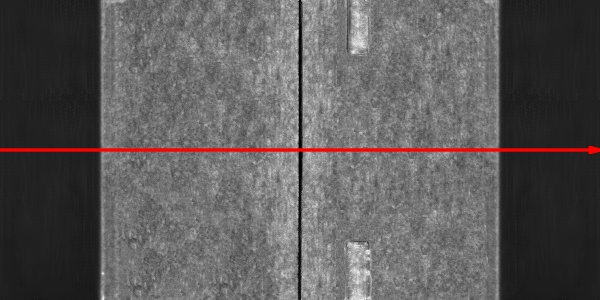
\includegraphics[width=\linewidth]{img/1DEdgeDetection/ridges_scan}
    \end{subfigure}%
    ~
    \begin{subfigure}[b]{\basicWidth}
		\smallProfile{img/1DEdgeDetection/ridges_profile.values}
    \end{subfigure}
    \caption{1D brightness profile of an image with strong ridge in its center.}
    \label{fig:RidgesProfile}
\end{figure}

\subsection{Ridge Operator}

\paragraph*{}
Ridges can be thought of as pairs of step edges of opposite polarity lying extremely close to each other. We could use this observation to propose a simple ridge detector operator adding together results of Forward Difference and Backward Difference operators:
\begin{eqnarray*}
R[i] & = & (S[i]-S[i-1])+(S[i]-S[i+1]) \\
	& = & 2S[i]-S[i-1]-S[i+1]
\end{eqnarray*}

\paragraph*{}
Such operator would be a discreet equivalent of the ridge operator proposed by Canny\cite{Canny86}, it has however two important drawbacks, pointed out by Subirana-Vilanova and Sung\cite{Subirana-VilanovaSung93}:

\begin{itemize}
	\item The operator has non-zero response for step edges, which can easily lead to false-positive errors.
	\item The quality of the detection strongly depends on the ridges having exactly 1 pixel in width, while in reality ridges usually appear as at least slightly wider.
\end{itemize}

\paragraph*{}
Both problems are illustrated by \reffig{RidgesNaiveResponse} - we can notice a high impulse response for step edges on the boundary of the object. Moreover, as the ridge in the original image has three pixels in width, it appears in the resulting profile as a pair of consecutive step edges.

\profileFigure
{
	\addProfileData{img/1DEdgeDetection/ridges_naive_operator.values}
}
{Naive ridge detection operator applied to the example profile.}
{RidgesNaiveResponse}

\paragraph*{}
The authors of \cite{Subirana-VilanovaSung93} suggest to solve the problem of high response to step edges by applying each half of the ridge operator separately and using the minimum of two responses.

\[
	R[i] = \min(S[i]-S[i-1],S[i]-S[i+1])
\]

\paragraph*{}
Such form of the operator is already feasible for narrow (one pixel wide) ridges. To successfully detect wider ridges we could define a general operator parametrized by the width of the ridge and the width of the reference margin as follows:

\begin{eqnarray*}
R[i] & = \min( & \\
	& & \overline{S[i..(i+Width)]}-\overline{S[(i-1-Margin)..(i-1)]}, \\
	& & \overline{S[i..(i+Width)]}-\overline{S[(i+1)..(i+1+Margin)])} \\
	& ) &
\end{eqnarray*}

where $\overline{S[a..b]}$ denotes the average of S values between $a$-th and $b$-th element, both inclusive.

\paragraph*{}
It should be noted that contrary to the edge detection operator which could be applied regardless of the polarity of edges being extracted, our ridge detection operator (because of the minimum function) works specifically for bright ridges. To extract dark ridges, analogous equation with maximum operator should be used.

\paragraph*{}
\reffig{RidgesProperResponse} demonstrates the outcome of using such operator on the example data from \reffig{RidgesProfile}. The maximum operator suppresses the magnitude of negative values (indicating possible ridge candidates) but amplifies the magnitude of positive values. For clarity the drawing was cropped to negative-y part.

\profileFigure
{
	\addProfileData{img/1DEdgeDetection/ridges_proper_operator.values}
}
{Amended ridge detection operator applied to the example profile.}
{RidgesProperResponse}

\paragraph*{}
Example results of ridge detection performed using such operator are demonstrated in \reffig{RidgesResults}.

\oneFigure
{img/1DEdgeDetection/ridges_result}
{Results of ridge detection.}
{RidgesResults}
{\basicWidth}

\subsection{Post-processing}

\paragraph*{}
All methods of post-processing of the extracted step edge points described in Step Edges section are applicable to ridges. 

\begin{refImpl}
Ridge detection algorithms are implemented in three \studio filters. All of them share common extraction logic, differing only in post-processing method applied to select the final outcome.
\begin{itemize}
	\item \filter{ScanMultipleRidges}{1DEdgeDetection} - returns all of the extracted ridges.
	\item \filter{ScanExactlyNRidges}{1DEdgeDetection} - selects the most prominent set of ridges of given cardinality.
	\item \filter{ScanSingleRidge}{1DEdgeDetection} - wrapper over previous filter which selects the single most prominent ridge.
\end{itemize} 
\end{refImpl}

\section{Stripes}

\paragraph*{}
Stripes are flat sections of brightness profile bounded by two step edges of opposite polarity. Such definition indicates that the problem of stripe detection heavily depends on the already discussed detection of step edges. 

\paragraph*{}
The concept of stripe is important mostly as a clear and succint means of formulation for a range of visual inspection tasks, wheareas it does not bring any novelties to the signal-processing aspect of the computation. Indeed, algorithms for stripe extraction firstly find the step edges in the profile (using previously described methods) and then process the results combining the extracted edges into stripes. 

\paragraph*{}
Next section summarizes two basic methods of combining the extracted step edges into stripes.

\subsection{Edge Processing}

\subsubsection{All Stripes}

\paragraph*{} As long as our goal is to maximize the number of constructed stripes, the problem can be solved quite efficiently. It can be easily proven that a simple $O(n)$ algorithm that greedily connects each closing edge with the first opening edge between already constructed stripes and the closing edge itself yields optimal results.

\subsubsection{N Stripes}

\paragraph*{}
The task is slightly more complicated if we know the desired number of stripes in advance and aim at maximizing the sum of strengths of step edges constituing the selected stripes. To solve such optimization problem in $O(n^2)$ time we can use a dynamic programming solution.

\paragraph*{}
Let us define a partial solution to the problem as follows:
\begin{description}
	\item \texttt{Best[Prefix][Count]} - sublist of the first \texttt{Prefix} step edges of alternating edge-polarities having \texttt{Count} elements that yields the biggest sum of edge strengths.
\end{description}

\paragraph*{}
Having computed the results for \texttt{Prefix} $=p$ we can compute the results for \texttt{Prefix} $=p+1$ in linear time - for each \texttt{Count} $=c$ we need to consider only two cases, either using the $p+1$-th step edge to extend the optimal result of \texttt{Best[p][count-1]} or not, in which case the result for the subproblem will be equal to \texttt{Best[p][count]}.

\begin{refImpl}
Stripe detection algorithms are implemented in three \studio filters. All of them share common extraction logic, differing only in post-processing method applied to select the final outcome.
\begin{itemize}
	\item \filter{ScanMultipleStripes}{1DEdgeDetection} - maximizes the number of returned stripes.
	\item \filter{ScanExactlyNStripes}{1DEdgeDetection} - constructs the most prominent set of stripes of given cardinality.
	\item \filter{ScanSingleStripe}{1DEdgeDetection} - wrapper over previous filter which selects the single most prominent stripe.
\end{itemize} 
\end{refImpl}
\section{Examples}

\paragraph*{}
In this section we will demonstrate a few industrial applications of 1D Edge Detection methods.

\subsection{Positioning}

\paragraph*{}
\textbf{1D Edge Detection} methods are commonly employed to determine locations of objects. Let us consider an image of a capsule on a production line demonstrated in \reffig{OneDEdgeDetectionPositioning}. We assume that the capsule is aligned with the axis of the image and we want to determine the range of x-coordinates occupied by the object.

\twoFigures
{img/1DEdgeDetection/positioning_edge_points}
{img/1DEdgeDetection/positioning_result}
{1D Edge Detection applied to determine capsule position along the x axis.}
{OneDEdgeDetectionPositioning}
{\basicWidth}

\paragraph*{}
As long as the background is plain and contrasting with object border, such problem can be solved easily regardless of the inner content of the object. \reffig{OneDEdgeDetectionPositioning} demonstrates the edge points detected along the horizontal scan line and visualisation of the resulting capsule position. The algorithm detects redundant, inner edges, but this does not pose a difficulty, as we only need the first and the last edge point of the returned list.

\subsection{Code Reading}

\paragraph*{}
One of the classic applications of stripe detection is reading of 1D data codes. Depending on the barcode format, we may\footnote{E.g. in case of codes from EAN/UPC family commonly used in trade.} or may not\footnote{E.g. in case of Pharmacode or Code128 standard.} know the number of bars the code is composed of - in the first case we may improve the robustness of the method using the post-processing routine for extracting the fixed number of strongest stripes which we have discussed before. In either case we expect the method to measure the width of the bars present in the image.

\oneFigure
{img/1DEdgeDetection/bars_res}
{1D Edge Detection applied to read the widths of 1D code bars.}
{OneDEdgeDetectionCodeReading}
{\basicWidth}

\paragraph*{}
It is interesting to note that the intercept theorem guarantees that we may scan the barcode at any orientation of the scan line, as long as its deviation from the barcode axis does not disrupt the stripe detection routine - the proportions of widths of the intersected bars are preserved under any orientation of the scan line.

\paragraph*{}
Once the widths of the bars are obtained they can be passed to a decoder for the specific barcode format to obtain the final reading.


%\subsection{Counting}

%\paragraph*{}
%Another popular application of \textbf{1D Edge Detection} is counting of the objects positioned along a path. Let us assume that we want to count the blades of a circular presented in \reffig{Blade}.

%\singleFigure
%{img/1DEdgeDetection/blade}
%{A circular saw blade to be inspected.}
%{Blade}
%{0.65}

%\paragraph*{}
%Such task may be solved by running a single edge detection scan along a circular path intersecting the blades. To produce the scan path we can use a straightforward \filter{CreateCirclePath}{PathBasics} filter. The built-in plugin will allow us to point \& click the required \param{inCircle} parameter, as demonstrated in \reffig{BladePlugin}.

%\singleFigure
%{img/1DEdgeDetection/blade_plugin}
%{Interactive selection of the circle parameter.}
%{BladePlugin}
%{0.5}

%\paragraph*{}
%The next step will be to pick the specific algorithm for the actual edge detection. As the objects being inspected appear as stripes in one-dimensional brightness profile and we do not know how many of them there are, the \filter{ScanMultipleStripes}{1DEdgeDetection} would be a right tool for the job.

%\paragraph*{}
%The program depicted in (...) solves the problem as expected (perhaps after increasing the inSmoothingStdDev from default of 0.6 to bigger value of 1.0 or 2.0) and detects all 30 blades of the saw.

%\twinFigure
%{img/1DEdgeDetection/blade_scan_area}
%{img/1DEdgeDetection/blade_results}
%{Scan area and the extracted stripes.}
%{BladeResults}
%{0.5}

